\chapter{Condizionamento dell'Ingresso}

%--------------------------------------------------------------------------------------------

\section{Convertitore Lineare-Esponenziale}

%--------------------------------------------------------------------------------------------

Vogliamo ora analizzare il circuto che soddisfa la specifica sulla modalità $1\ V/Octave$
dell'ingresso, ovvero il circuito in grado di convertire una tensione lineare in una
esponenziale.

Il circuito utilizzato è molto diffuso in questo tipo di applicazioni, si può infatti
trovare in molti siti di DIY come quello di René Schmitz \cite{expo_converter}, personaggio
molto noto tra gli appassionati di sintetizzatori musicali fai-da-te.

%--------------------------------------------------------------------------------------------

\subsection*{Analisi del Circuito}

%--------------------------------------------------------------------------------------------

Per l'applicazione si sfrutta la caratteristica esponenziale intrinseca del transistor
bipolare, ovvero:

\begin{equation}\label{transistor_current}
    I_e\approx I_c=I_se^{\left(\frac{V_{be}}{V_T}-1\right)}
    \approx I_se^{\left(\frac{V_{be}}{V_T}\right)}\ [A]
\end{equation}

\begin{figure}[H]
    \centering
    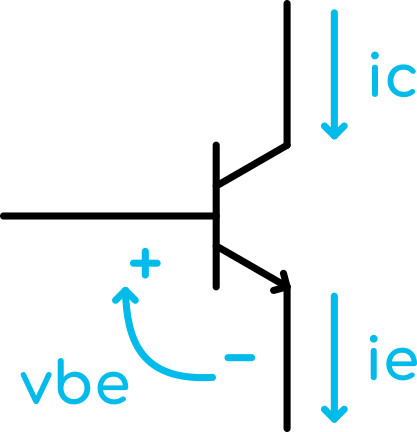
\includegraphics{circuits/single_transistor_circuit.png}
    \caption{BJT}
    \label{bjt}
\end{figure}

dove $V_T$ (o potenziale termico) e $I_s$ (o corrente di saturazione) sono variabili in
funzione della temperatura. Nella nostra analisi $V_T$ verrà considerato di valore costante
pari a $26\ mV$, mentre si rimuove dall'equazione $I_s$ collegando una coppia di transistor
(idealmente nello stesso chip, in modo che siano il più possibile simili tra loro e ù
termicamente accoppiati) in configurazione differenziale:

\begin{figure}[H]
    \centering
    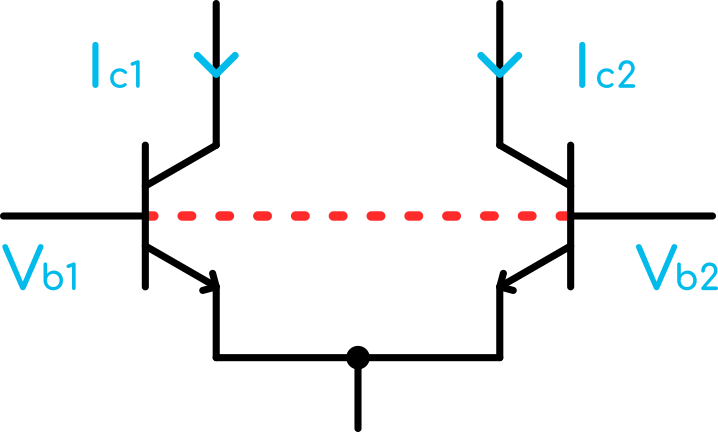
\includegraphics{circuits/differential_pair_circuit.png}
    \caption{Coppia differenziale a BJT}
    \label{differential_pair_circuit}
\end{figure}

per la quale possiamo scrivere la seguente relazione:

\begin{equation}\label{differential_pair}
    \frac{I_{c2}}{I_{c1}}=\frac{I_s e^{\left(\frac{V_{be2}}{V_T}\right)}}{I_s e^{\left(\frac{V_{be1}}{V_T}\right)}}
    \qquad
    \rightarrow
    \qquad
    I_{c2}=I_{c1}e^{\left(\frac{V_{be2}-V_{be1}}{V_T}\right)}=I_{c1}e^{\left(\frac{V_{b2}-V_{b1}}{V_T}\right)}\ [A]
\end{equation}

in cui risulta evidente che la dipendenza da $I_s$ viene completamente rimossa.

A questo punto, rinominiamo le grandezze come segue:

\begin{equation}\label{renamed_differential_pair}
    \left\{ \begin{aligned}
        I_{c2} & = I_{freq} \\
        I_{c2} & = I_{ref}
    \end{aligned} \right.
    \qquad
    \rightarrow
    \qquad
    I_{freq}=I_{ref}e^{\left(-\frac{V_{b1}}{V_T}\right)}\ [A]
\end{equation}

e aggiungiamo al circuito

\begin{itemize}
    \item un amplificatore invertente per portare $V_{in}$ in un range appropriato alla base
          di $Q_1$ (operazionale di sinistra, figura \ref{exponential_converter_circuit})
          \begin{equation}\label{amplifier}
              V_{b1}=-V_{in}\cdot s=
              -V_{in}\cdot\frac{R_f}{R_{in}}\cdot\frac{\%R_{pot}+R}{R_{pot}+R}\ [V]
          \end{equation}
    \item un anello di controllo per mantenere la corrente di riferimento $I_{ref}$ costante
          (operazionale centrale, figura \ref{exponential_converter_circuit})
          \begin{equation}\label{iref}
              I_{ref}=\frac{V_{HR}-V_{LR}}{R_{ref}}\ [A]
          \end{equation}
    \item un convertitore corrente-tensione al collettore di $Q_2$ (operazionale di destra,
          figura \ref{exponential_converter_circuit})
          \begin{equation}\label{ivconv}
              V_{exp}=I_{freq}\cdot R_{conv}\ [V]
          \end{equation}
\end{itemize}

ottenendo quindi il seguente circuito con la relativa relazione ingresso/uscita:

\begin{figure}[H]
    \centering
    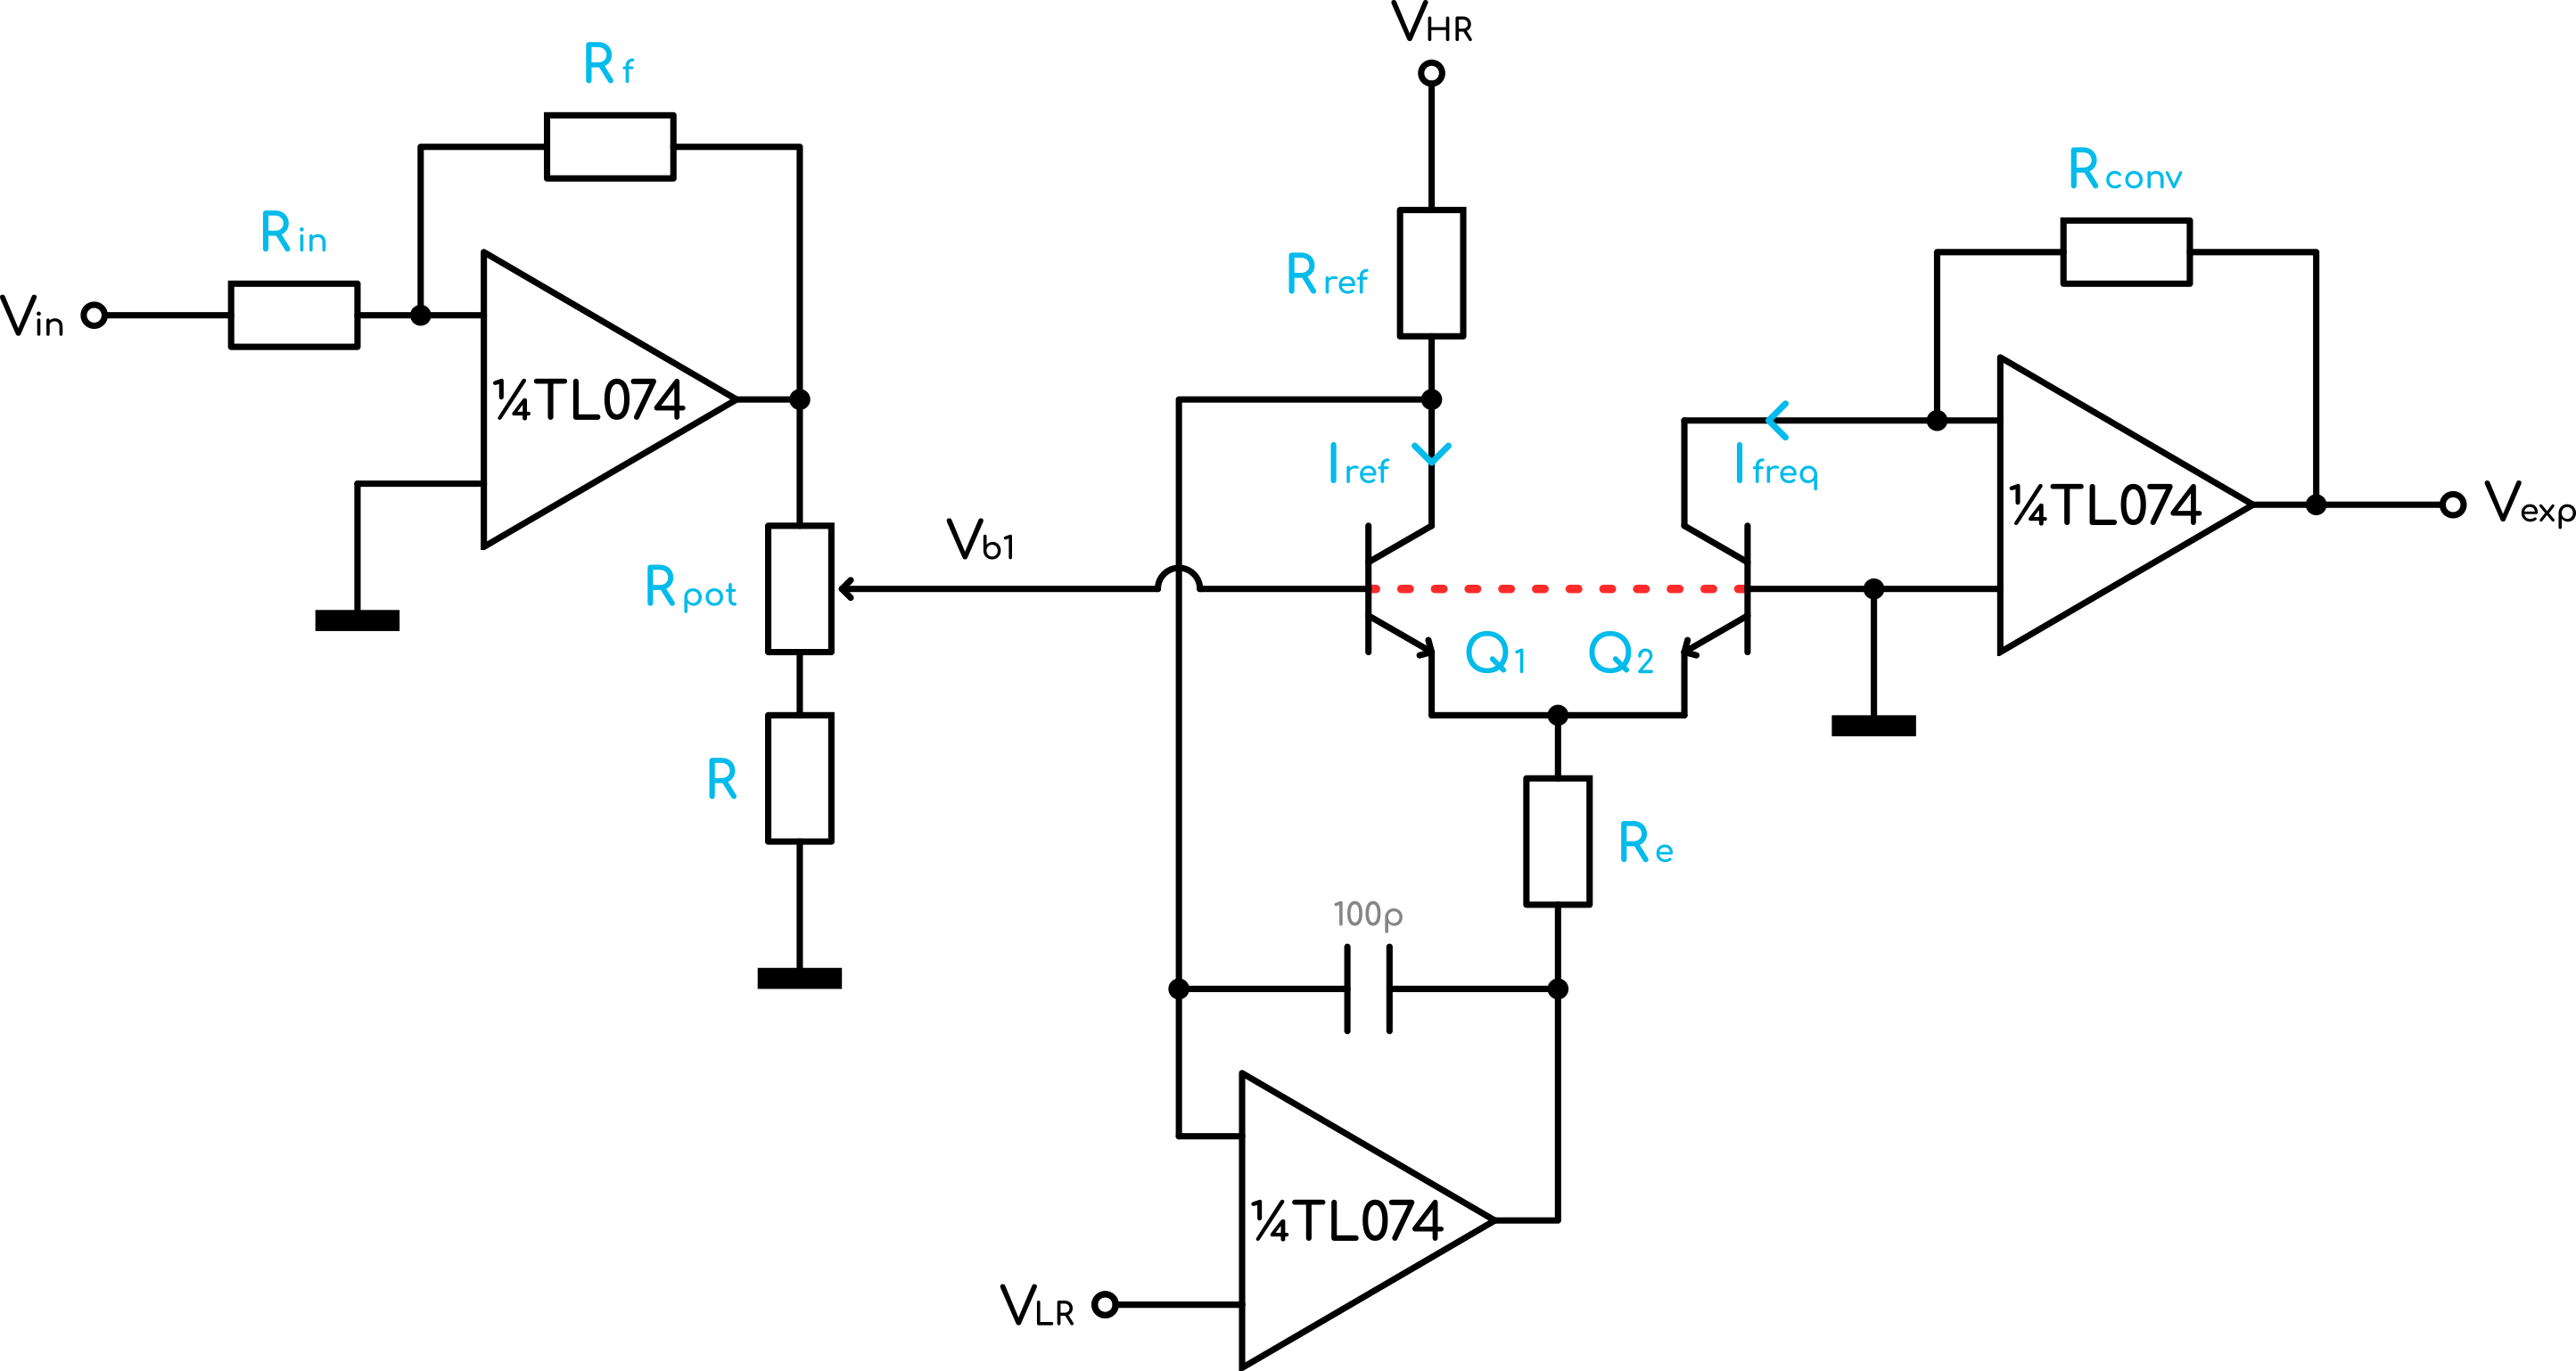
\includegraphics{circuits/exponential_converter_circuit.png}
    \caption{Schema elettrico del convertitore tensione lineare-esponenziale}
    \label{exponential_converter_circuit}
\end{figure}

\begin{equation}\label{expo_converter}
    V_{exp}=R_{conv}\cdot \frac{V_{HR}-V_{LR}}{R_{ref}}e^{\left(\frac{s\cdot V_{in}}{V_T}\right)}\ [V]
\end{equation}

%--------------------------------------------------------------------------------------------

\subsection*{Dimensionamento e Scelta dei Componenti}

%--------------------------------------------------------------------------------------------

Passiamo quindi al dimensionamento dei componenti, in modo da imporre al circuito il
comportamento voluto.

Come prima cosa calcoliamo il valore del guadagno $s$ dell'amplificatore invertente.
Si vuole:

\begin{equation}\label{iref_doubling}
    I_{freq}=I_{ref}e^{\left(\frac{s\cdot V_{in}}{V_T}\right)}
    \qquad
    \xrightarrow{+\Delta V_{in}}
    \qquad
    2I_{freq}=I_{ref}e^{\left(\frac{s\cdot(V_{in}+\Delta V_{in})}{V_T}\right)}
\end{equation}

qundi un raddoppio della corrente $I_{freq}$ per ogni variazione $\Delta V_{in}=1\ V$.
Allora possiamo riscrivere la relazione nel seguente modo:

\begin{equation}\label{s1}
    \frac{2I_{freq}}{I_{freq}}=
    \frac{I_{ref}e^{\left(\frac{s\cdot(V_{in}+\Delta V_{in})}{V_T}\right)}}
    {I_{ref}e^{\left(\frac{s\cdot V_{in}}{V_T}\right)}}
    \
    \rightarrow
    \
    2=e^{\left(\frac{s\cdot\Delta V_{in}}{V_T}\right)}
    \
    \rightarrow
    \
    ln(2)=\frac{s\cdot\Delta V_{in}}{V_T}
    \
    \rightarrow
    \
    s=\frac{V_T\cdot ln(2)}{\Delta V_{in}}
\end{equation}

\begin{equation}\label{s2}
    s=\frac{26\ mV\cdot 0.6931}{1\ V}\approx0.018\approx\frac{1}{55.5}
\end{equation}

\begin{equation}\label{s3}
    s=\frac{R_f}{R_{in}}\cdot\frac{\%R_{pot}+R}{R_{pot}+R}
    =\frac{2\ k\Omega}{100\ k\Omega}\cdot\frac{440\ \Omega}{490\ \Omega}
    \approx 0.018
\end{equation}

quindi:

\begin{itemize}
    \item $R_f = 2\ k\Omega$;
    \item $R_{in} = 100\ k\Omega$;
    \item $R_{pot} = 100\ \Omega$;
    \item $R = 390\ \Omega$;
\end{itemize}

Scegliamo anche $R_{conv}=3.3\ k\Omega$, per avere come massimo valore di corrente
$I_{freq} = 3\ mA$ ($V_{exp}\approx+10\ V$ in uscita dal convertitore corrente-tensione),
in corrispondenza di una tensione di ingresso $V_{in}=+8\ V$. Da qui possiamo quindi calcolare
il valore di $I_{ref}$:

\begin{equation}\label{iref_calc}
    I_{ref}=I_{freq}e^{\left(-\frac{s\cdot V_{in}}{V_T}\right)}
    =0.003e^{\left(-\frac{0.018\cdot8}{0.026}\right)}
    \approx11.8\ \mu A
\end{equation}

Impostando quindi $V_{HR}=+12\ V$ e $V_{LR}=0\ V$ calcoliamo $R_{ref}$:

\begin{equation}\label{rref_calc}
    R_{ref}=\frac{V_{HR}}{I_{ref}}=\frac{12}{11.8\cdot10^{-6}}\approx 1\ M\Omega
\end{equation}

Ora, poichè la corrente massima a scorrere in $R_e$ vale $I_{ref}+I_{freq}\approx3\ mA$
potremmo scegliere anche $R_e=R_{conv}=3.3\ k\Omega$. In questo modo sommando le cadute di
potenziale $V_{R_{ref}}$, $V_{ce\_sat\_1}$ e $V_{R_e}$, saremmo dentro il limite dei valori
di alimentazione, ottenendo $\approx 22.2\ V\ < 24\ V= 2V_{cc}$.

Se però andiamo a calcolare la caduta di potenziale ai capi di $R_e$ corrispondente a $V_{in}=0\ V$,
ovvero:

\begin{equation}\label{vre}
    V_{R_e}=R_e(I_{ref}+I_{freq})=3.3\cdot10^3\cdot23.6\cdot10^{-6}\approx77.9\ mV
\end{equation}

notiamo che un valore di resistenza maggiore aumenterebbe la linearità del circuito per bassi
livelli di $V_{in}$, in quanto la caduta di potenziale sul resistore ha modulo maggiore e
risulta meno influenzata dal rumore. Si modifica allora il circuito cosicché che la
resistenza di emettitore sia variabile in modo non-lineare, a seconda della corrente
richiesta in uscita. Questo è reso possibile sostituendo ad $R_e$ un parallelo tra due resistori
di diverso valore, di cui quello più piccolo collegato in serie ad un diodo, l'elemento che
si occuperà effettivamente di modificare il valore di resistenza.

\begin{figure}[H]
    \centering
    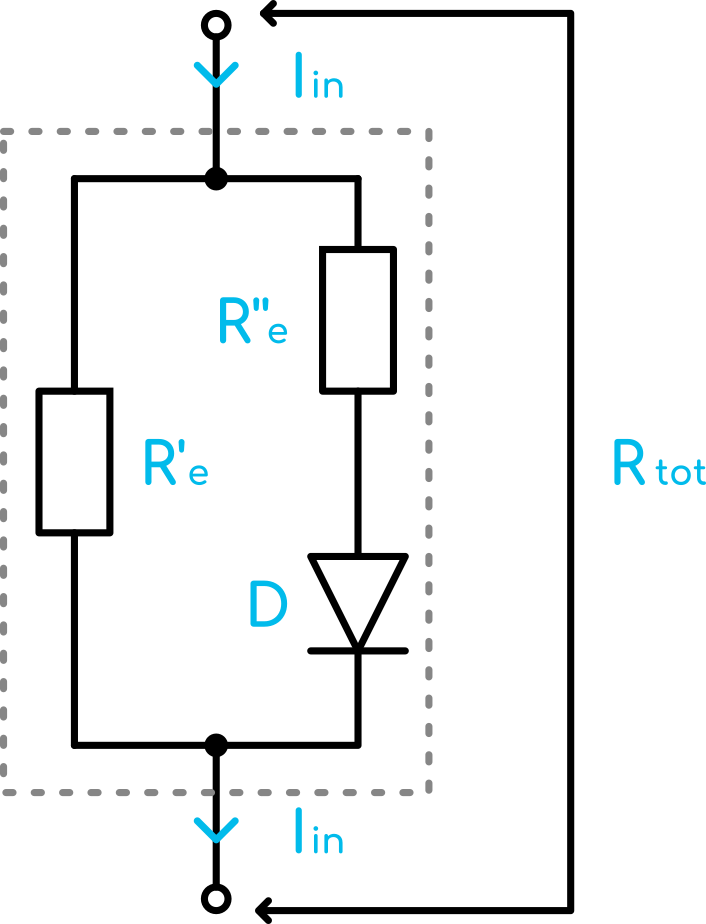
\includegraphics{circuits/Rtot_circuit.png}
    \caption{Schema elettrico del resistore variabile}
    \label{Rtot_circuit}
\end{figure}

Come resistori possiamo scegliere qualsiasi valore, purchè non comporti la saturazione
dell'operazionale e si aggiri comunque attorno al $k\Omega$. Si scelgono $R_e'=10\ k\Omega$
e $R_e''=1.2\ k\Omega$.

\begin{equation}\label{rtot}
    R_{tot} =
    \left\{
    \begin{array}{lr}
        R_e'        & \text{con diodo spento, ovvero } I_{ref}+I_{freq}\leq\frac{V_d}{R_e'} \\
        R_e'//R_e'' & \text{con diodo acceso, ovvero } I_{ref}+I_{freq}>\frac{V_d}{R_e'}
    \end{array}
    \right.
\end{equation}

Per quanto riguarda i componenti, ancora una volta gli amplificatori operazionali utilizzati
sono dei TL074, mentre si sceglie un MPQ3904 \cite{mpq3904} per i transistor, chip che
ospita 4 unità al proprio interno, e vista la disponibilità, il diodo in figura viene
sostituito con uno dei 4 transistor del chip configurato come diodo.

\begin{figure}[H]
    \centering
    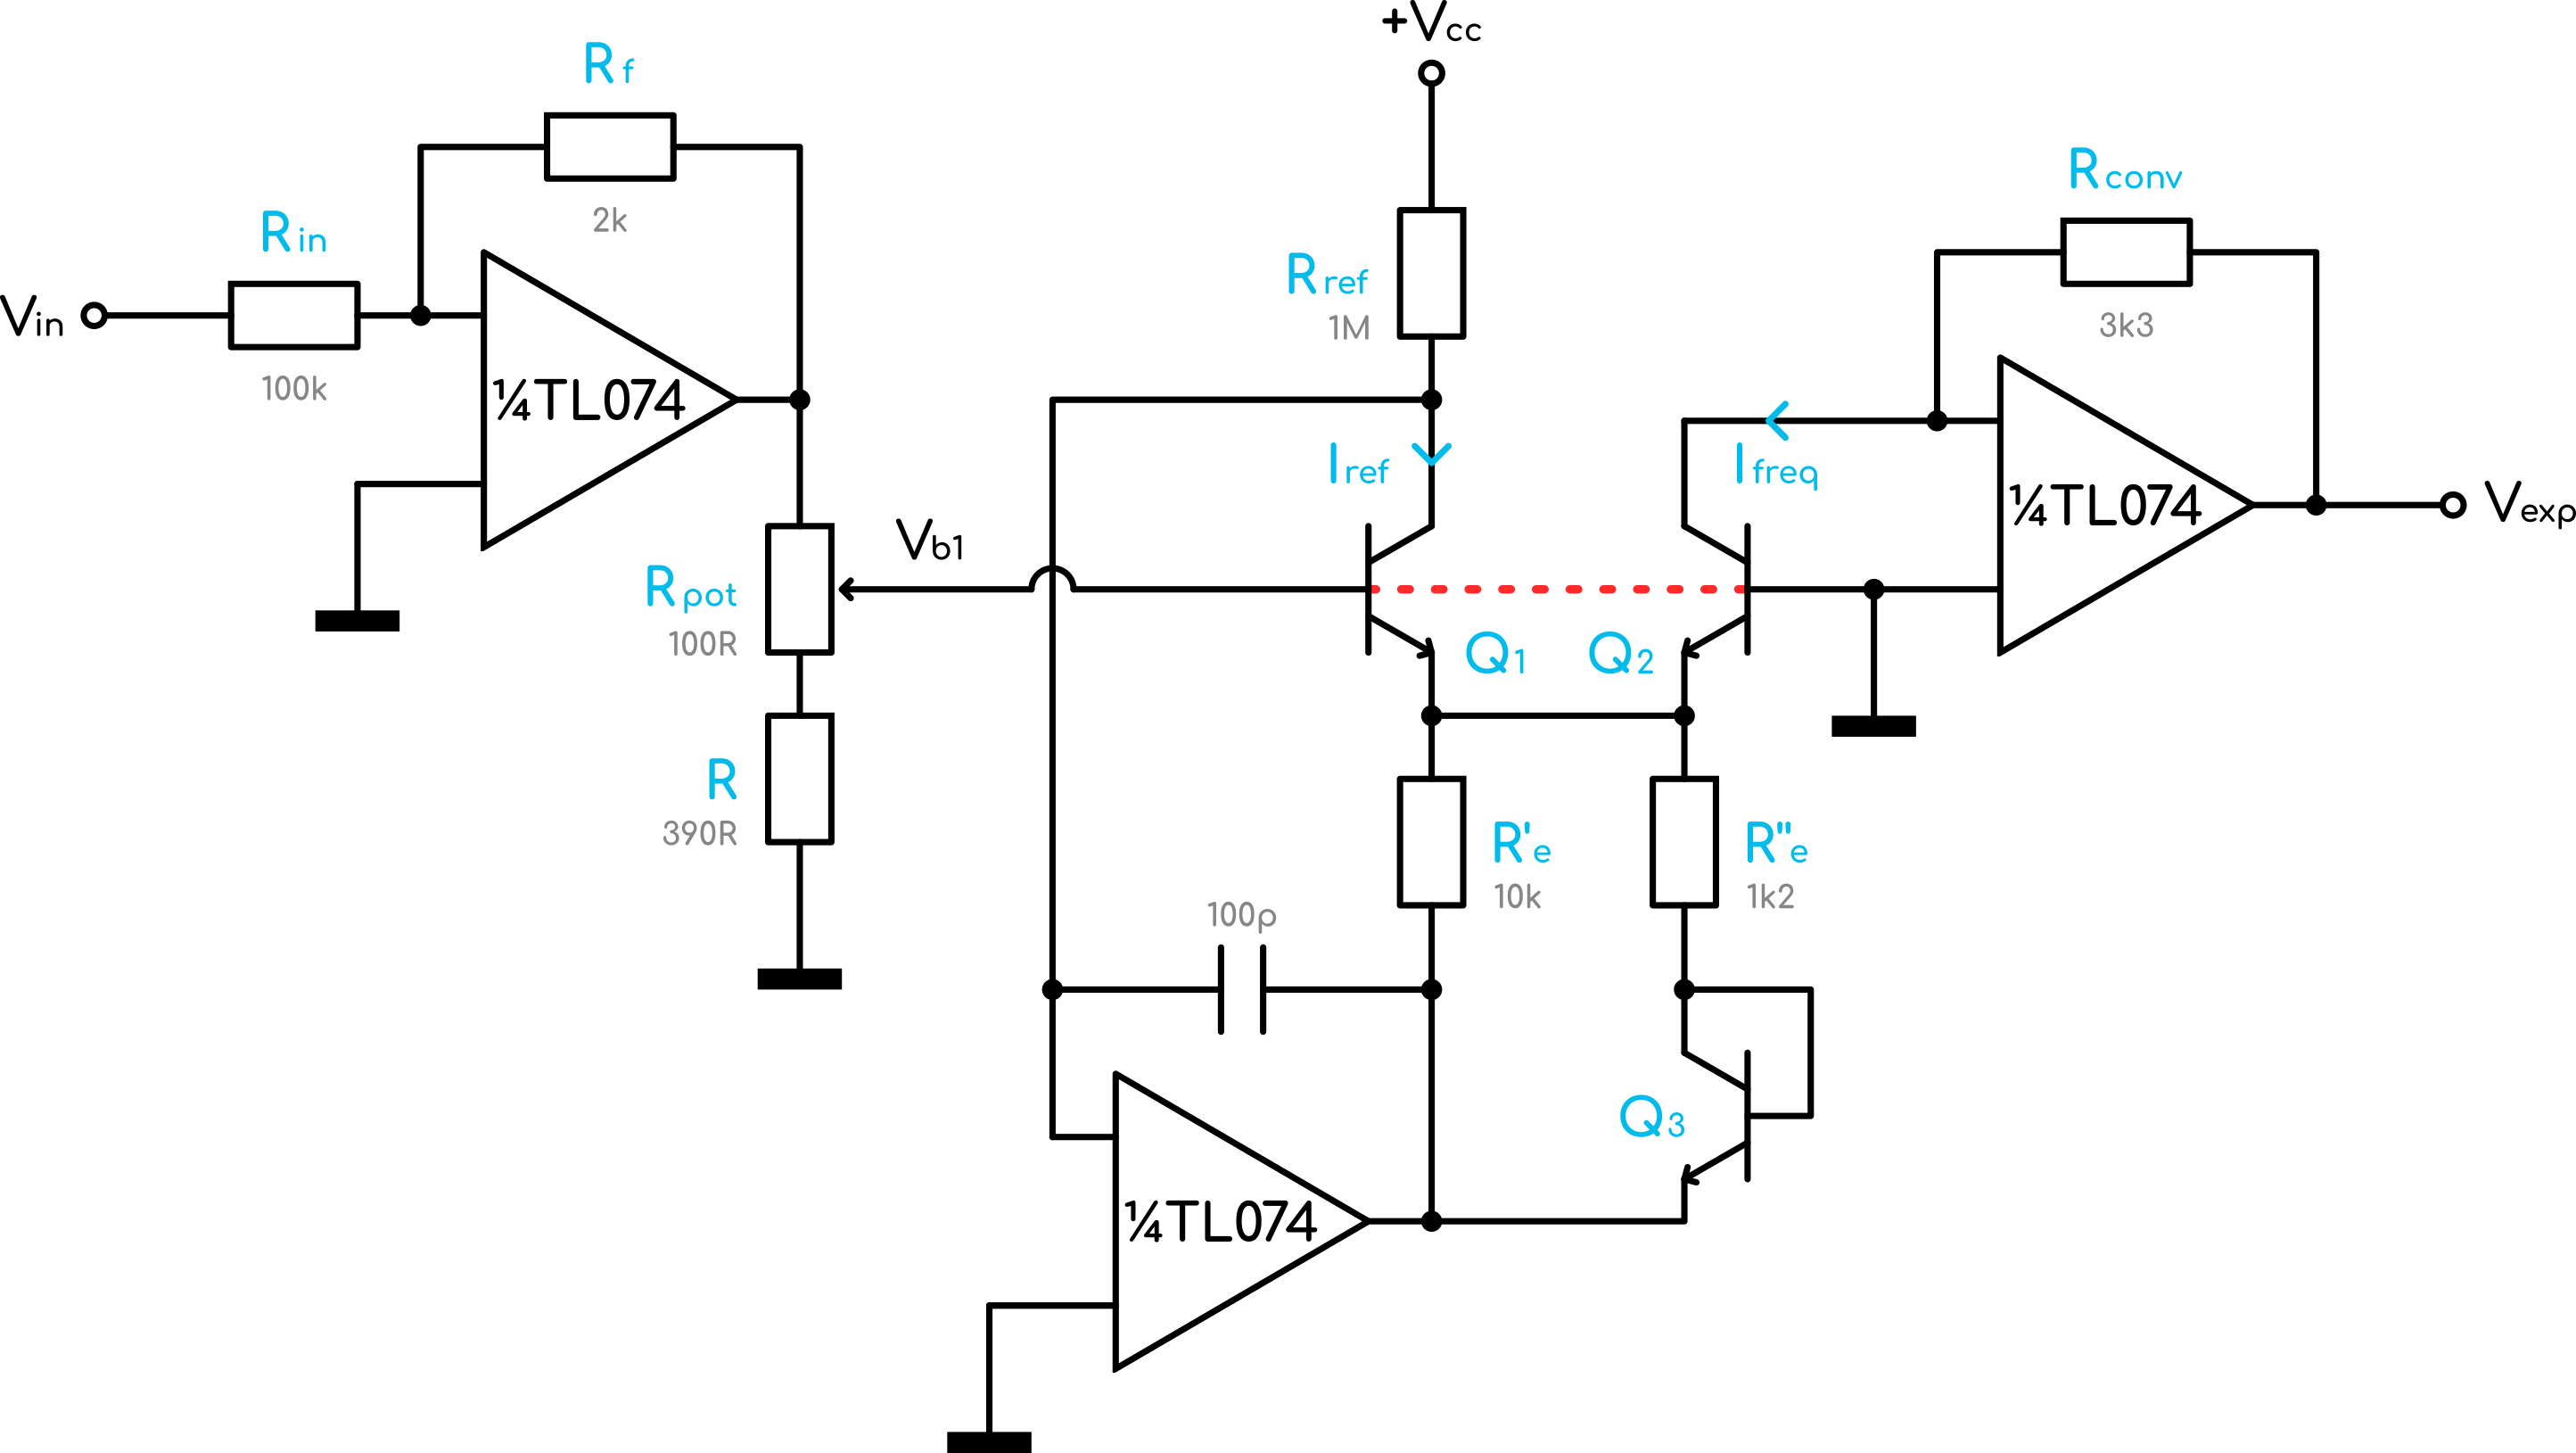
\includegraphics{circuits/complete_exponential_converter_circuit.png}
    \caption{Schema elettrico del convertitore tensione lineare-esponenziale completo}
    \label{complete_exponential_converter_circuit}
\end{figure}

%--------------------------------------------------------------------------------------------

\subsection*{Risultati Pratici e Misure}

%--------------------------------------------------------------------------------------------

Analizziamo ora il comportamento del circuito.

% dati, tabelle e grafici

%--------------------------------------------------------------------------------------------

\section{Somma di più Ingressi}

%--------------------------------------------------------------------------------------------

Per fare in modo che possa essere utilizzato un segnale in tensione come modulante (ingresso
LFO), si aggiunge un resistore uguale a $R_{in}$ all'ingresso invertente dell'amplificatore,
modificando quindi la relazione \ref{amplifier} nel seguente modo:

\begin{equation}
    V_{b1}=-s\cdot\sum_0^n{V_{n}}\ [V]
\end{equation}

% figura

rendendo quindi l'amplificatore un sommatore invertente. Si noti che non c'è un limite al
numero di ingressi che è possibile aggiungere.

%--------------------------------------------------------------------------------------------

\section{Clipper}

%--------------------------------------------------------------------------------------------

Come visto dalla formula \ref{expo_converter}, la tensione in ingresso $V_{in}$ deve essere di
valore positivo per avere una tensione in uscita positiva, e volendo inserire nel circuito
un nodo sommatore per avere la possibilità di utilizzare un segnale in tensione come modulante,
dobbiamo assicurarci che $V_{b1}$ non diventi mai positiva (il segno viene invertito
dall'amplificatore). Si aggiunge quindi un blocco raddrizzatore, realizzato con un diodo e
un operazionale, che compenserà per la caduta di tensione sul diodo. Lo schema utilizzato
viene riportato in figura %\ref{}.

% figura

Quindi in uscita si avrà la stessa tensione in ingresso se negativa, mentre un valore molto
prossimo a $0$ se positiva.

\begin{equation}\label{clipper}
    V_{out} =
    \left\{
    \begin{array}{lr}
        V_{in} & \text{con} V_{in}\le0 \\
        0      & \text{con} V_{in}>0
    \end{array}
    \right.
\end{equation}

Il diodo utilizzato per lo scopo è un 1N4148 \cite{1n4148}, un comunissimo diodo per piccoli
segnali, e l'operazionale sempre un TL074.

%--------------------------------------------------------------------------------------------

\subsection*{Risultati Pratici e Misure}

%--------------------------------------------------------------------------------------------

Verificando il circuito appena discusso vediamo che si comporta esattamente come desiderato.

% immagini grafici e tabelle

%--------------------------------------------------------------------------------------------
